\documentclass[11pt]{article}
\usepackage[final]{acl}
\usepackage{times}
\usepackage{latexsym}
\usepackage[T1]{fontenc}
\usepackage[utf8]{inputenc}
\usepackage{microtype}
\usepackage{graphicx}
\usepackage{booktabs}
\usepackage{multirow}
\usepackage{adjustbox}
\usepackage{amsmath}
\graphicspath{{figures/}{../figures/}}

\newcommand{\Sup}{\textsc{support}}
\newcommand{\Con}{\textsc{contradict}}
\newcommand{\Nei}{\textsc{nei}}

\title{Copies, Conflicts and Broken Parses: How Corpus Defects Affect\\Retrieval-Augmented Claim Verification}

\author{Likhith Venkata Sai Manikanta Nalla \\
  Independent researcher \\
  \texttt{likhith.nalla1@gmail.com}}

\begin{document}
\maketitle

\begin{abstract}
Retrieval-augmented systems inherit the quality of the collection they search, but the
effect of specific defects is rarely measured in isolation. We inject four controlled defects into the
SciFact corpus (near-duplicate copies, stale copies with flipped findings, broken parsing, and chunking)
at 10--50\% of the gold-evidence documents, and measure, claim by claim, how they change retrieval and
the verdicts of four verifiers: two zero-shot LLMs (Qwen2.5 1.5B and 3B) and an NLI cross-encoder used
off the shelf or fine-tuned. Results are repeated over five corruption seeds and three training seeds and
replicated on Climate-FEVER. Copies push the gold document out of first place (dense recall@1 from 0.74
to 0.53 at 50\% stale copies) but barely change verification, whereas broken parsing is almost invisible
to retrieval yet costs correct answers for both LLMs and for the fine-tuned verifier on every seed. Flipped copies move the fine-tuned
verifier towards \textsc{contradict}, and on one-sentence Climate-FEVER records cost it many correct answers
(up to 55 lost against 14 gained) and make it more often confidently wrong; both LLMs largely ignore them.
Single-sentence chunks make the fine-tuned verifier less accurate and more confident. Monitoring retrieval
alone would rank these defects in the wrong order of harm.
\end{abstract}

\section{Introduction}

Retrieval-augmented generation \citep[RAG;][]{lewis2020rag} answers a question from documents
retrieved out of a collection, so its answers can be no better than that collection. Real collections
are imperfect: documents are duplicated across sources, older versions sit next to newer ones that
contradict them, PDF parsing truncates or scrambles text, and chunking splits documents into pieces of
varying size. Robustness studies of RAG usually vary what reaches the reader, for instance by adding
irrelevant or counterfactual passages to its context \citep{cuconasu2024noise,chen2024rgb,xie2024chameleon},
rather than the collection the retriever searches. Practitioners, however, control the collection,
and need to know which of its defects are worth cleaning.

We ask how much each of four common defects, on its own, changes retrieval and the final answer. We
use claim verification because it has labels for both the answer (does the evidence support or
contradict the claim?) and the evidence (which documents), so a defect's effect can be traced from
retrieval to the verdict. Defects are injected under control, one type and rate at a time, into an
otherwise unchanged corpus, with every model, prompt and threshold held fixed, so any change in the
results comes from the corpus. Our contributions:

\begin{itemize}
\setlength\itemsep{0pt}
\item A seeded corruption tool for four defect types (near-duplicates, stale copies with flipped
  findings, broken parsing, chunking) that logs every change, and a pipeline that regenerates and
  verifies each corrupted corpus from its seed.
\item Paired, claim-level measurements on SciFact \citep{wadden2020scifact} for two retrievers, a
  reranker and four verifiers, repeated over five corruption seeds and three verifier training seeds,
  and replicated on Climate-FEVER \citep{diggelmann2020climatefever}.
\item Evidence that retrieval metrics rank the defects in the wrong order of harm, that stale copies
  matter only to verifiers that read their context closely, and that small chunks make a fine-tuned
  verifier confidently wrong.
\end{itemize}

All code, per-claim predictions, corruption manifests and fine-tuned models are public.\footnote{%
\url{https://github.com/Likhithvenkatanalla/rag-dq-benchmark}; archived at
\url{https://doi.org/10.5281/zenodo.23314458}.}

\section{Related Work}

\paragraph{Robustness of retrieval-augmented models.}
Language models are easily distracted by irrelevant context \citep{shi2023distracted}, use the middle
of long contexts poorly \citep{liu2024lost}, and can be trained to ignore irrelevant passages
\citep{yoran2024robust}. RGB \citep{chen2024rgb} tests noise robustness, negative rejection and
counterfactual robustness of RAG readers, and \citet{cuconasu2024noise} find that random documents in
the context can even help. These studies manipulate the reader's context directly; we manipulate the
collection and let the retriever decide what reaches the reader.

\paragraph{Knowledge conflicts.}
\citet{longpre2021conflicts} substitute entities in passages to create conflicts with a model's
parametric knowledge, and \citet{xie2024chameleon} show that LLMs readily accept coherent conflicting
evidence. Our stale copies create conflicts \emph{within} the collection: the original and a flipped
copy are both retrievable, as when outdated and current versions of a document coexist.

\paragraph{Duplicates and data quality.}
Near-duplicates are pervasive in web-scale text and deduplication improves language-model training
\citep{lee2022dedup}. Retrieval benchmarks such as BEIR \citep{thakur2021beir} evaluate retrievers
across clean collections; we hold the task fixed and vary the collection's quality.

\paragraph{Claim verification.}
FEVER \citep{thorne2018fever}, SciFact \citep{wadden2020scifact} and Climate-FEVER
\citep{diggelmann2020climatefever} pair claims with evidence and a verdict, which makes the path from
evidence to answer measurable.

\section{Setup}

\subsection{Data}
\paragraph{SciFact} pairs expert-written scientific claims with 5,183 abstracts. We evaluate on the 300
dev claims (124 \Sup, 64 \Con, 112 \Nei); 188 have gold evidence, among 184 distinct gold abstracts.
The 809 train claims, disjoint from dev, are used only for training and threshold tuning.

\paragraph{Climate-FEVER} pairs real-world climate claims with five Wikipedia sentences each, labelled by
annotators. We build a closed corpus from all 5,240 distinct evidence sentences (each a record titled
with its article), close in size to SciFact, and drop the 154 \textsc{disputed} claims, leaving 1,381
claims (654 \Sup, 253 \Con, 474 \Nei). A claim's gold records are its evidence sentences labelled with
the claim's own verdict (907 claims have at least one). No model is trained on Climate-FEVER.

\subsection{Pipeline}
\paragraph{Retrieval.} BM25 \citep{robertson2009bm25} over whitespace tokens, and dense retrieval with
BGE-small-en-v1.5 \citep{xiao2023cpack} and exact cosine search \citep{johnson2019faiss}. Recall@$k$ is
the share of a claim's gold records found in the top $k$, averaged over claims with evidence.

\paragraph{Verification.} A verifier reads the claim with the top-3 dense-retrieved records and outputs
\Sup, \Con\ or \Nei. \emph{Qwen-1.5B} and \emph{Qwen-3B} are Qwen2.5-1.5B/3B-Instruct
\citep{qwen2024qwen25}, zero-shot with greedy decoding, instructed to answer with one word.
\emph{NLI zero-shot} is the cross-encoder \texttt{nli-deberta-v3-xsmall} \citep{he2023debertav3} as
released, and \emph{NLI fine-tuned} is the same model fine-tuned for 3 epochs on 1,123 SciFact train
pairs (gold abstracts with their labels; cited abstracts of claims without evidence and the top
non-gold BM25 abstract of each claim with evidence as \Nei), trained with three seeds. An NLI verifier
scores each (claim, record) pair; the claim takes the higher of the maximum \Sup\ and \Con\
probabilities over its three records, or \Nei\ if neither reaches a threshold tuned for macro-F1 on 20\%
of the train claims held out from training (never on dev).

\paragraph{Reranking.} A MiniLM cross-encoder \citep{nogueira2019rerank}, as released or fine-tuned on
SciFact train, reorders the dense top-10 before verification.

\subsection{Defects}
Each defect is applied to a share (10, 25 or 50\%) of the gold-evidence records, so that it reaches the
evaluated claims; claims and labels never change.
\begin{itemize}
\setlength\itemsep{0pt}
\item \textbf{Duplicate} adds a near-copy of the record (one sentence dropped if there are more than two,
  about 5\% of words deleted, one adjacent word pair swapped per sentence).
\item \textbf{Stale} adds a copy whose directional findings are flipped by rule
  (\emph{increased}$\leftrightarrow$\emph{decreased}, \emph{higher}$\leftrightarrow$\emph{lower},
  ``is associated'' $\rightarrow$ ``is not associated'', \dots; for Climate-FEVER also
  \emph{warming}$\leftrightarrow$\emph{cooling}, \emph{rise}$\leftrightarrow$\emph{fall}, \dots).
  Copies with nothing to flip are identical to the original; we analyse flipped copies separately.
\item \textbf{Parse} replaces the record with a broken parse: truncated at 30--60\% of its length,
  sentences scrambled, or OCR-style character noise.
\item \textbf{Chunk} splits every SciFact abstract into records of 1, 3 or 5 sentences (not applicable to
  one-sentence Climate-FEVER records).
\end{itemize}
A copy is a different document: retrieving it does not count as retrieving the gold record. A chunk
counts as its parent abstract.

\subsection{Statistics}
All runs on a dataset share the same claims, so comparisons are paired: for each claim we record
whether the answer went from right to wrong (\emph{lost}) or wrong to right (\emph{gained}) relative to
the clean corpus, and report both counts with an exact McNemar test \citep{mcnemar1947}. We run many
such tests without correction, so we treat as findings only effects whose direction repeats across
corruption seeds and, for the fine-tuned verifier, training seeds.

\section{Results on SciFact}

\subsection{Clean baseline}
Dense retrieval beats BM25 at every cut-off (recall@1 0.744 vs.\ 0.615; recall@10 0.957 vs.\ 0.883).
Qwen-1.5B reaches 0.557 accuracy and 0.502 macro-F1 (majority class: 0.413 and 0.195) but answers
\Sup\ for 200 of 300 claims. The fine-tuned NLI verifier reaches 0.650 / 0.680 / 0.667 for its three
training seeds, each significantly above Qwen-1.5B (lost/gained 32/60, 36/73, 35/68; $p \le 0.005$).
Untuned, the NLI model reaches only 0.353. Doubling the LLM closes the gap: Qwen-3B reaches 0.667 accuracy and 0.655
macro-F1, significantly above Qwen-1.5B (34 lost, 67 gained; $p=0.001$) and level with the fine-tuned
verifier, without any training; its answers are spread evenly over the three labels (109 \Sup, 96 \Con,
95 \Nei).

\subsection{Retrieval}

\begin{table}[t]
\centering\small
\setlength\tabcolsep{4pt}
\begin{adjustbox}{max width=\columnwidth}
\begin{tabular}{lccc}
\toprule
Corpus & BM25 & Dense & + rerank \\
\midrule
clean & 0.615 & 0.744 & 0.805 \\
duplicate 10/25/50\% & .594/.541/.463 & .689/.668/.604 & .774/.751/.644 \\
stale 10/25/50\% & .583/.530/.466 & .691/.622/.551 & .752/.657/.571 \\
parse 10/25/50\% & .615/.599/.578 & .744/.734/.739 & .795/.799/.758 \\
chunk 5/3/1 sent. & .583/.590/.520 & .749/.742/.762 & .803/.818/.784 \\
\bottomrule
\end{tabular}
\end{adjustbox}
\caption{SciFact recall@1 (188 claims with evidence; corruption seed 0). Recall@10 is unchanged by
copies (0.883 BM25, 0.957 dense).}
\label{tab:retrieval}
\end{table}

Copies push the gold abstract out of first place in proportion to their rate
(Table~\ref{tab:retrieval}, Figure~\ref{fig:retrieval}) while recall@10 does not change: a copy usually
sits just above its original. Over five corruption seeds, dense recall@1 at 50\% falls to $0.584 \pm 0.019$
(duplicates) and $0.528 \pm 0.031$ (stale), against 0.744 clean.
The fine-tuned reranker lifts clean recall@1 to 0.805 and recovers part of the duplicate loss but little
of the stale loss: a flipped copy is as relevant to the claim as its original, so a relevance model
cannot tell them apart. Broken parsing removes documents from BM25's reach (recall@10 0.845 at 50\%) but
barely affects dense retrieval, and chunking hurts BM25 but not dense retrieval.

\begin{figure*}[t]
\centering
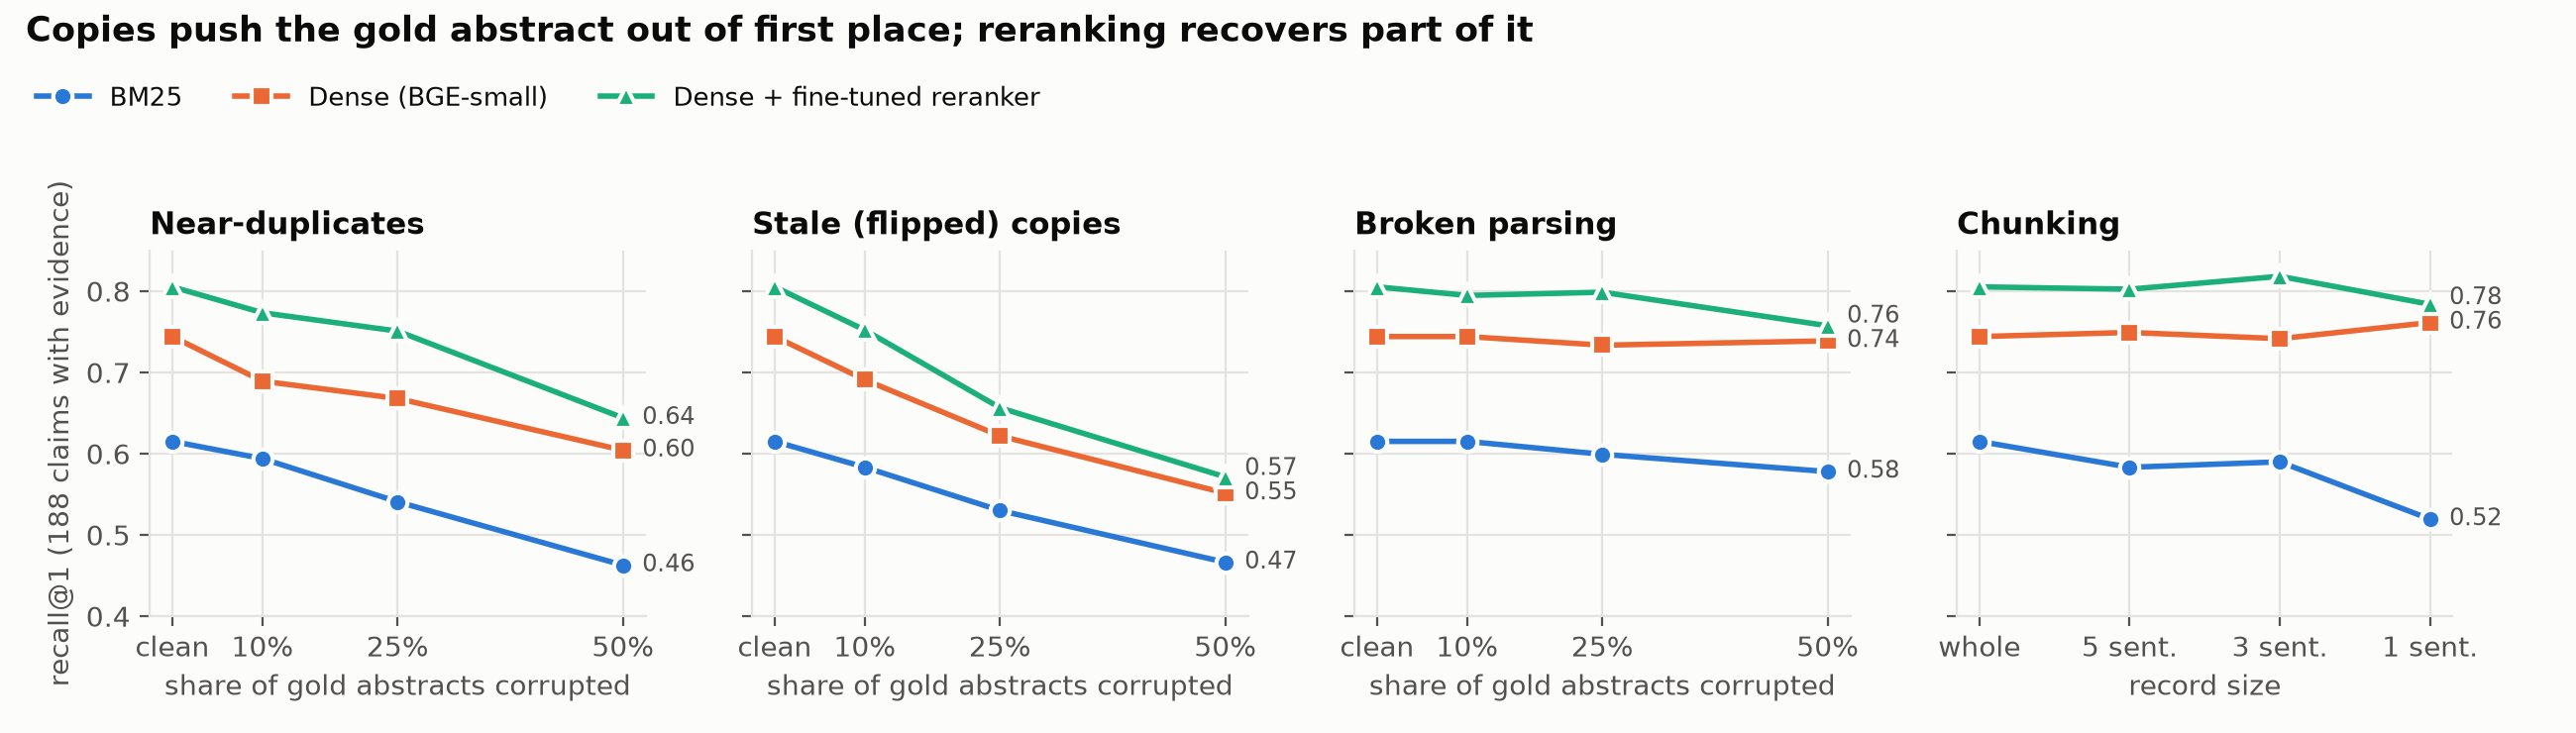
\includegraphics[width=\textwidth]{fig2_retrieval.png}
\caption{SciFact recall@1 by corruption level for BM25, dense retrieval and dense retrieval with the
fine-tuned reranker (corruption seed 0).}
\label{fig:retrieval}
\end{figure*}

\subsection{Verification}

\begin{table}[t]
\centering\small
\setlength\tabcolsep{4pt}
\begin{adjustbox}{max width=\columnwidth}
\begin{tabular}{lccc}
\toprule
Setting & Dense R@1 & NLI acc. & Lost / gained \\
\midrule
clean & 0.744 & 0.650 & -- \\
dup.\ 10\% & .704 (.015) & .649 (.003) & 3 / 1 \\
dup.\ 25\% & .665 (.026) & .653 (.005) & 5 / 10 \\
dup.\ 50\% & .584 (.019) & .657 (.009) & 7 / 18 \\
stale 10\% & .696 (.004) & .647 (.009) & 8 / 3 \\
stale 25\% & .624 (.011) & .646 (.010) & 16 / 10 \\
stale 50\% & .528 (.031) & .649 (.005) & 23 / 22 \\
parse 10\% & .744 (.004) & .643 (.007) & 11 / 1 \\
parse 25\% & .736 (.008) & .641 (.006) & 18 / 4 \\
parse 50\% & .733 (.010) & .631 (.006) & 41 / 13 \\
\bottomrule
\end{tabular}
\end{adjustbox}
\caption{SciFact over five corruption seeds (mean, sd): dense recall@1, accuracy of the fine-tuned
verifier (training seed 0), and claims lost / gained relative to clean, summed over the seeds.}
\label{tab:seeds}
\end{table}

\begin{table}[t]
\centering\small
\setlength\tabcolsep{3.5pt}
\begin{adjustbox}{max width=\columnwidth}
\begin{tabular}{lccc}
\toprule
Corpus & Qwen-1.5B & NLI zero-shot & NLI fine-tuned \\
\midrule
clean & 0.557 & 0.353 & 0.666 (.015) \\
dup.\ 10/25/50\% & .543/.547/.557 & .360/.367/.353 & .670/.670/.677 \\
stale 10/25/50\% & .553/.550/.560 & .353/.357/.347 & .672/.661/.656 \\
parse 10/25/50\% & .550/.547/.530 & .357/.347/.340 & .664/.658/.647 \\
chunk 5/3/1 & .543/.573/.583 & .390/.353/.333 & .667/.631/.573 \\
\bottomrule
\end{tabular}
\end{adjustbox}
\caption{SciFact verification accuracy (300 claims; corruption seed 0). Fine-tuned: mean over three
training seeds (sd on clean).}
\label{tab:verification}
\end{table}

Accuracy changes are small for most defects (Table~\ref{tab:verification}, Figure~\ref{fig:verification}),
so we read them claim by claim.

\paragraph{Broken parsing costs verification.} With five corruption seeds, the seed-0 fine-tuned verifier lost more
correct answers than it gained in 14 of the 15 parse runs and gained more in none (Table~\ref{tab:seeds}):
41 lost against 13 gained over the five 50\% corpora, 18 against 4 at 25\%. No single run is significant
at $p<0.05$ (the largest has 12 lost, 4 gained), which is why repetition matters here: under no effect,
a net loss on all five seeds has probability $1/32$ for each rate. Qwen-1.5B shows the same direction
(8 lost, 0 gained at 50\%, $p=0.008$), as do all three training seeds on corruption seed 0. Qwen-3B, too, loses more than it gains at 25\% (5 vs.\ 2) and 50\% (13 vs.\ 7).
Every verifier we tested is hurt by broken parsing in the same direction.

\paragraph{Single-sentence chunks hurt the fine-tuned verifier}, consistently across training seeds
(0.573 mean accuracy; lost/gained 58/38, 65/32 and 64/34, $p=0.052$, $0.001$, $0.003$). It was trained
on whole abstracts; 5-sentence chunks do not hurt it, and neither Qwen model is hurt by chunking.

\paragraph{Duplicates do not change verification}, despite their effect on retrieval: the gold abstract
is still in the top 3 for nearly as many claims (gold-in-context rate 0.872 clean, 0.867 at 50\%), and a
near-copy carries the same evidence. Over five seeds the fine-tuned verifier gained slightly more answers
than it lost at 25--50\% (12 lost, 28 gained in total), consistent with no harm.

\paragraph{Reranking barely changes verification.} Verifying from the fine-tuned reranker's top-3 moves
accuracy by 0 to +2.3 points across the 13 corpora, with no run changing significantly: the gold abstract
is usually already within the dense top-3, and its position there matters little to the verifier.

\begin{figure*}[t]
\centering
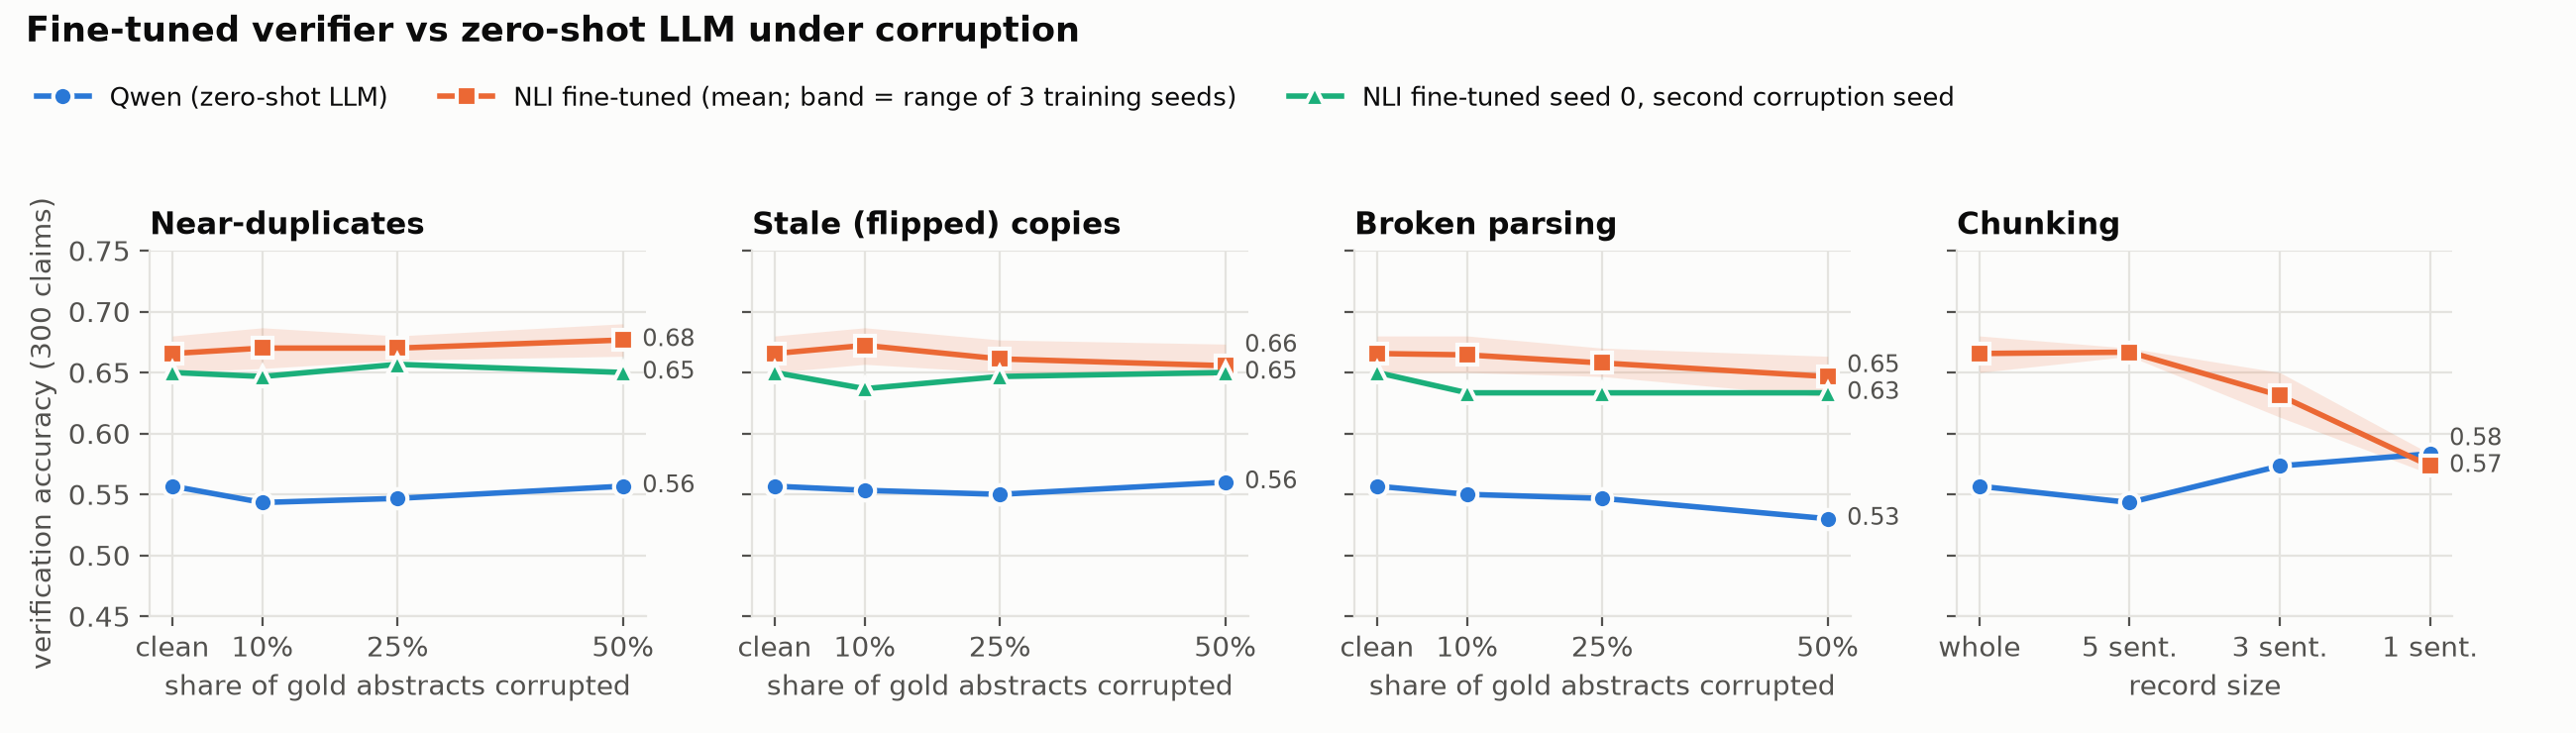
\includegraphics[width=\textwidth]{fig1_verification.png}
\caption{SciFact verification accuracy by corruption level. The orange band spans the three fine-tuned
training seeds; the green line is the seed-0 verifier on corruption seed 1 (its own clean value is 0.650).}
\label{fig:verification}
\end{figure*}

\subsection{Conflicting evidence}

To isolate genuinely conflicting evidence we keep only claims whose top-3
context held a stale copy whose findings were actually flipped, and compare them with the same claims on
the clean corpus. At 50\% on corruption seed 0, 78 claims qualify. The fine-tuned verifier changed its
answer on 13, 19 and 16 of them (training seeds 0/1/2), and 11, 15 and 12 of those changes went to \Con;
Qwen-1.5B changed 6 and moved 1 to \Con, consistent with its \Sup\ bias. Qwen-3B, despite matching the fine-tuned verifier's accuracy, behaves like the
smaller LLM: %QWEN3B_STALE_NUMBERS% Over five
corruption seeds the pattern is stable: of 48 changed answers at 50\%, 35 moved to \Con. Claims whose
context held only unflipped copies never changed answer for the NLI verifier. Yet no verifier's accuracy
changes significantly: the fine-tuned verifier is misled on some claims and helped on others (23 lost,
22 gained over five seeds at 50\%), and flipped copies do not make it more often confidently wrong
(55 such answers on these claims clean, 56 with stale copies). The count rose on two corruption seeds
and fell on three, so the increase we reported earlier for a single seed was not robust.

\subsection{Calibration}

We give each NLI answer a confidence (for \Sup\ or \Con, the highest probability
of that label over the three records; for \Nei, one minus the highest \Sup\ or \Con\ probability) and
compare it with correctness; the Qwen models give no probabilities. The fine-tuned verifier is
overconfident even on clean data: mean confidence 0.75--0.80 against accuracy 0.65--0.68, expected
calibration error \citep[ECE;][]{guo2017calibration} 0.14--0.18, and 8--11\% of claims answered wrongly
with confidence of at least 0.9 (\emph{confidently wrong}). Copies and broken parses barely change this.
Small chunks do: with 1-sentence records confidence rises while accuracy falls, ECE roughly doubles
(0.31--0.32 for all three training seeds) and 18--22\% of claims are confidently wrong
(Figure~\ref{fig:confwrong}).

\begin{figure}[t]
\centering
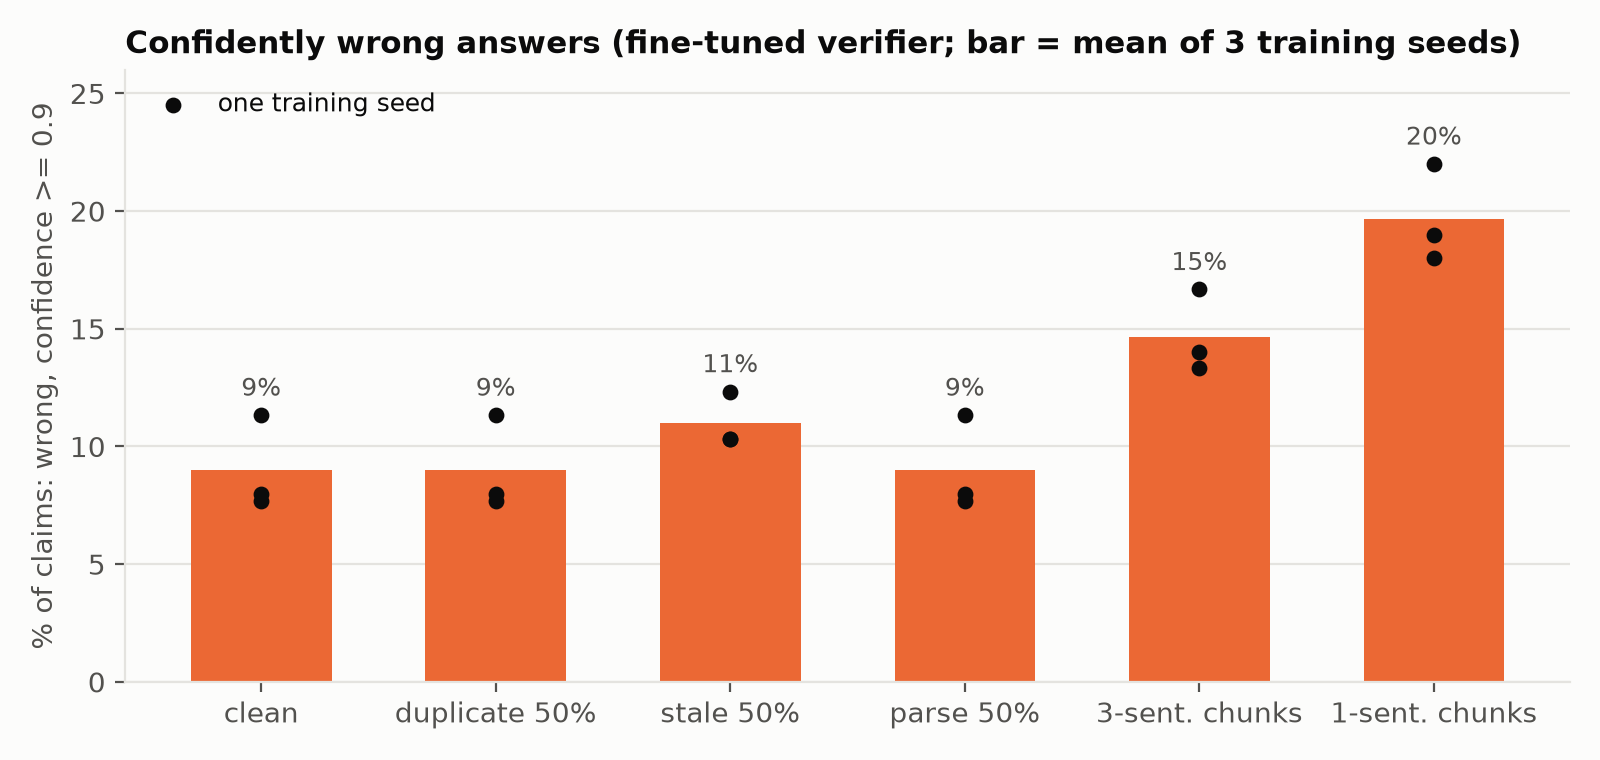
\includegraphics[width=\columnwidth]{fig4_confident_wrong.png}
\caption{SciFact: share of claims answered wrongly with confidence $\ge 0.9$ by the fine-tuned verifier
(bar: mean of three training seeds; dots: seeds).}
\label{fig:confwrong}
\end{figure}

\section{Replication on Climate-FEVER}

\begin{table*}[t]
\centering\small
\setlength\tabcolsep{5pt}
\begin{adjustbox}{max width=\textwidth}
\begin{tabular}{lcccccc}
\toprule
& \multicolumn{2}{c}{Retrieval} & \multicolumn{2}{c}{Qwen-1.5B} & \multicolumn{2}{c}{NLI fine-tuned (SciFact)} \\
\cmidrule(lr){2-3}\cmidrule(lr){4-5}\cmidrule(lr){6-7}
Corpus & Gold in top-3 & Dense R@10 & Acc. & Lost / gained & Acc.\ (3 seeds) & Lost / gained at 50\% (seeds 0/1/2) \\
\midrule
clean & 0.534 & 0.522 & 0.508 & -- & 0.458 & -- \\
duplicate 10 / 25 / 50\% & .526 / .517 / .494 & .515 / .499 / .486 & .511 / .520 / .516 & 5/9, 4/21, 21/33 & .459 / .457 / .456 & 29/24, 25/21, 24/24 \\
parse 10 / 25 / 50\% & .531 / .515 / .504 & .509 / .495 / .475 & .510 / .511 / .506 & 3/6, 7/12, 21/19 & .457 / .452 / .458 & 38/32, 27/30, 28/31 \\
stale 10 / 25 / 50\% & .528 / .516 / .496 & .516 / .502 / .489 & .509 / .511 / .508 & 4/6, 11/15, 26/27 & .453 / .446 / .433 & 55/14, 46/16, 48/15 \\
\bottomrule
\end{tabular}
\end{adjustbox}
\caption{Climate-FEVER (1,381 claims; corruption seed 0). Gold in top-3: share of claims with evidence
whose dense top-3 holds a gold sentence. Lost / gained: claims right on the clean corpus and wrong on
the corrupted one, and the reverse.}
\label{tab:climate}
\end{table*}

Climate-FEVER differs from SciFact in ways that make it a demanding replication: records are single
Wikipedia sentences, claims come from the web rather than from experts, and no verifier was trained on it.
Retrieval is much harder (a gold sentence reaches the dense top-3 for 53\% of claims with evidence, against
87\% on SciFact), and both verifiers are weak: Qwen-1.5B reaches 0.508 accuracy (majority class 0.474)
with \Nei\ for only 89 claims, and the SciFact-trained NLI verifier transfers poorly, at 0.458 (0.450--0.468)
and significantly below Qwen-1.5B for every training seed ($p \le 0.039$). The findings that replicate are
therefore the ones that do not depend on absolute accuracy (Table~\ref{tab:climate}).

\paragraph{Stale copies hurt the NLI verifier, much more than on SciFact.} At 25\% and 50\% each training
seed lost far more correct answers than it gained (at 50\%: 55/14, 46/16 and 48/15, all $p<0.001$), and
accuracy fell monotonically with the rate for every seed. On claims with a flipped copy in their top-3
(356 at 50\%), the verifier changed 84--101 answers, about half of them to \Con, and became more often
confidently wrong for all three seeds (98$\rightarrow$119, 95$\rightarrow$120, 79$\rightarrow$107).
Qwen-1.5B again barely reacted (26 lost, 27 gained). A one-sentence record leaves no other evidence to
outweigh a flipped finding, which plausibly explains why the effect is stronger than on SciFact.

\paragraph{Copies displace gold records without hurting verification.} Duplicates and stale copies lower the
gold-in-top-3 rate by about four points at 50\%, yet duplicates leave accuracy essentially unchanged
(the fine-tuned verifier moves by at most 0.4 points; Qwen-1.5B even gains at 25\%, 4 lost against 21 gained).

\paragraph{Broken parsing has no consistent effect here.} With one-sentence records, a third of the parse
corruptions (sentence scrambling) change nothing, and truncation leaves part of a short sentence; the
lost/gained counts point in both directions across verifiers and seeds.

\section{Discussion}

\paragraph{Retrieval metrics can rank defects in the wrong order.} On SciFact,
duplicates and stale copies cause the largest drops in recall@1 but no reliable change in verification,
because the verifier reads the top 3 and the gold abstract rarely leaves it. Broken parsing shows the
opposite: retrieval barely notices it, yet it is the defect that most consistently costs correct answers,
for both LLMs and for the fine-tuned verifier across all its training and corruption seeds, because the verifier receives a truncated or
scrambled version of the right abstract. Monitoring retrieval alone would put these defects in the wrong
order; answer-level evaluation on a corrupted copy of one's own collection is cheap and does not.

\paragraph{Whether conflicting evidence matters depends on the reader.} The fine-tuned NLI verifier reads each
record closely and reacts to flipped copies: on SciFact it moves answers to \Con\ without a net loss, and on
Climate-FEVER, where a record is one sentence, it loses many correct answers and becomes confidently wrong more
often. Both zero-shot LLMs largely ignore the flipped copies, including Qwen-3B, which is as accurate as the
fine-tuned verifier on clean SciFact. Relevance-based reranking does not help, since a flipped copy is as
relevant as its original. Detecting version conflicts needs signals beyond relevance, such as dates,
provenance, or deduplication before indexing.

\paragraph{Chunk size interacts with the verifier's training.} The fine-tuned verifier, trained on whole
abstracts, degrades on single sentences and grows more confident while doing so. Chunking should match the
format a verifier was trained on, and a verifier's confidence should not be trusted outside that format.

\section*{Limitations}

Effects of a few claims out of 300 (SciFact) are within noise, and the McNemar
$p$-values are not corrected for multiple comparisons; our findings rest on repetition across corruption
seeds, training seeds, verifiers and datasets. Qwen-3B and the Climate-FEVER runs use one corruption seed.
Stale copies are produced by rule-based word substitution, so they may read less naturally than real
outdated documents, and some copies have nothing to flip (about 20\% on SciFact, 32\% on Climate-FEVER), which we
handle by analysing flipped copies separately. Defects target gold-evidence records, which makes their effect
on evaluated claims visible but does not model how defects are distributed in real collections. All models
are small (BGE-small, Qwen2.5 up to 3B, DeBERTa-v3-xsmall) because every experiment ran on free CPU runners;
larger readers may react differently, and we did not study generation beyond a one-word verdict.

\section*{Ethics and Reproducibility Statement}
SciFact and Climate-FEVER are public research datasets; they are downloaded from their official
releases and not redistributed. All experiments ran on free CPU runners of GitHub Actions; the
workflows that produced every number are in the repository, and each corrupted corpus is regenerated
from its seed and checked against the committed manifest. Code was developed with AI assistance
(Claude); every reported number comes from runs whose outputs are in the repository.

\bibliography{references}

\end{document}
